\chapter{Antriebsstrang}
\fancyfoot[C]{Lackner}

<<<<<<< HEAD

%% Übersicht %%%%%%%%%%%%%%%%%%%%%%%%%%%%%%%%%%%%%%%%%%%%%%%
\section{Übersicht}
Die Hauptaufgabe des Antriebssystems ist die Umwandlung der, vom Akkumulator zur Verfügung gestellten, elektrischen Energie in die kinetische Antriebsenergie. Diese tritt zuerst rotatorisch am Motor auf und wird zunächst über das Direkt-Getriebe umgeformt bzw. auf die passende Drehzahl gebracht, anschließend wird die Rotationsenergie mithilfe des Hinterrades auf die Straße übertragen und das ganze Motorrad beschleunigt. Neben dem Antrieb des Motorrades hat die Motorsteuerung noch weitere Bedeutung als Steuereinheit, sie fungiert als Bindeglied zwischen dem Human-Computer Interacting System und den elektrischen Anforderungen an das Gesamtsystem.


\subsection{Grundfunktionen des Systems}
Die geplanten Aufgaben des Antriebssystems lassen sich grob in zwei Grundfunktionen einteilen:

\begin{itemize}
	\item \textbf{Der Antrieb} 
	\\ \medskip Translation ist eine Grundfunktion eines jeden Verkehrsmittels.
	\\ Durch die Umwandlung der elektrischen Energie in kinetische Energie erfährt 
	\\ das gesamte System eine Beschleunigung in Fahrtrichtung.
	\medskip
	\item \textbf{Die Steuereinheit}
	\\ \medskip Steuerung und Kommunikation mit anderen Betriebsmitteln,
	\\ realisiert durch In- und Outputs, Datenübetragung mithilfe des CAN-Buses. 
\end{itemize}

\vspace{5mm}

Um auf die einzelnen Details des Antriebssystems besser eingehen zu können, unterscheiden wir zwischen dem Hardwareaufbau und dem Softwareaufbau des Antriebssystems.

\newpage



%% Hardwareaufbau %%%%%%%%%%%%%%%%%%%%%%%%%%%%%%%%%%%%%%%%%%%%%%%
\section{Hardwareaufbau des Antriebssystems}
Der grundsätzliche Hardwareaufbau des Antriebssystems lässt sich in zwei galvanisch getrennte Stromkreise und die mechanische Umsetzung unterscheiden:
\\[5mm]
\begin{itemize}
	\item \textbf{Mechanische Umsetzung (Kraftübertragung und Montage)} 
	\\ \medskip Umfasst das Getriebe und die Befestigung aller Komponenten am Rahmen.
	\medskip
	\item \textbf{Der Laststromkreis}
	\\ \medskip Beinhaltet die Verbindung des Motorcontrollers mit dem Motor und dem Akkumulator.
	\medskip
	\item \textbf{Der Steuerstromkreis}
	\\ \medskip Beinhaltet alle elektrischen Verbindungen, welche mithilfe des 35-poligen
	\\ Niederleistungs-Steckers mit dem Motorcontroller verbunden sind.
\end{itemize}

\newpage



%% Mechanische Umsetzung %%%%%%%%%%%%%%%%%%%%%%%%%%%%%%%%%%%%%%%%%%%%%%% 
\subsection{Mechanische Umsetzung}
Die Fertigung des Getriebes und die Montage der einzelnen Betriebsmittel wurde vollständig von Tobias Schmeisser übernommen.


\newpage



%% Der Laststromkreis %%%%%%%%%%%%%%%%%%%%%%%%%%%%%%%%%
\subsection{Der Laststromkreis}
Der Laststromkreis beinhaltet alle leistungsführenden Betriebsmittel des Antriebssystems. Hierbei unterscheiden wir zwischen den zwei wichtigsten Grundfunktionen:
\\[5mm]
\begin{itemize}
	\item \textbf{Elektrische Energieübertragung}
	\\ \medskip Umfasst die elektrische Verbindung von Motor, Motorcontroller und Akkumulator. 			\\ Realisiert durch einfache Leitungen, um Leistungen übertragen zu können.
	\medskip
	\item \textbf{Schutz der Komponenten vor Beschädigungen (Leitungsschutzorgane)}
	\\ \medskip Beinhaltet eine Schmelzsicherung zum Schutz vor Überströmen und ein 					\\ Hochleistungs-Relais, um im Fehlerfall den Laststromkreis öffnen zu können und damit eine  		
	\\ galvanische Trennung des Antriebs und der Energieversorgung gewährleisten zu können.
\end{itemize}
\vspace{5mm}

Im folgenden Bild ist der Grundaufbau des Laststromkreises ausführlich beschrieben:
\vspace{2mm}
\\R1 ... Vorladewiderstand
\\F1 ... Schmelzsicherung
\\S4.1 ... Hauptschütz (Hochleistungs-Relais)
\\S4.2 ... Vorladeschütz
\vspace{5mm}
\begin{figure}[H]
	\begin{center}
		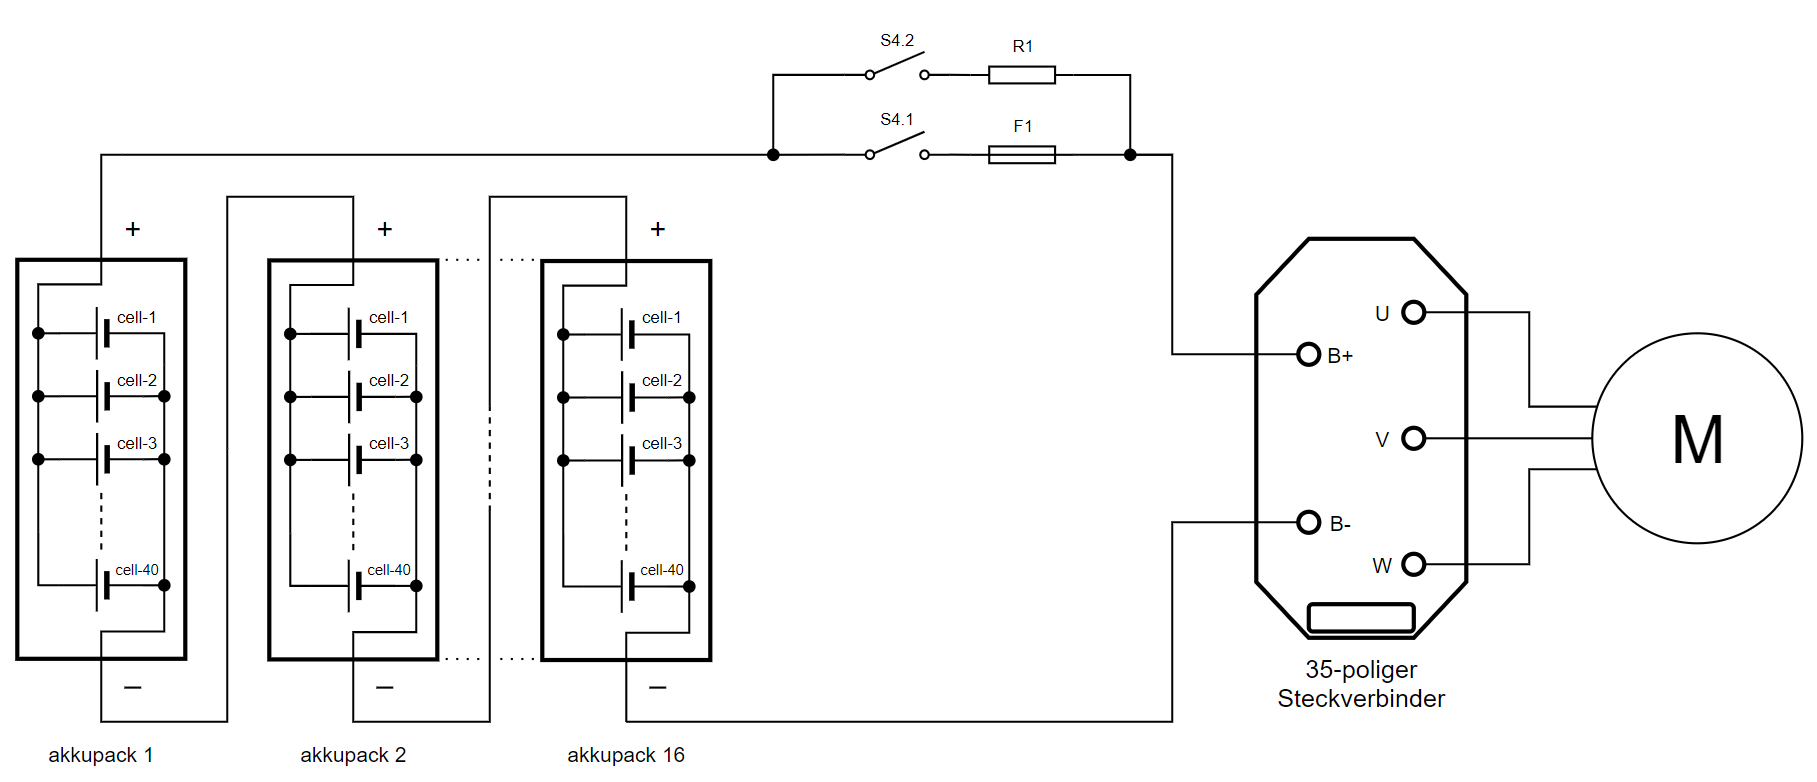
\includegraphics[scale=0.5]{figures/Antrieb/Antrieb_Laststromkreis.png}
		\caption{Grundaufbau des Laststromkreises}
	\end{center}
\end{figure}

\newpage



%% Elektrische Energieübertragung %%%%%%%%%%%%%%%%%%%%%%%%%%%%%%%%%
\subsubsection{Elektrische Energieübertragung}
Um die benötigte elektrische Energie übertragen zu können, müssen die Leitungen an den Leistungsverbrauch des Verbrauchers (Motor) angepasst werden. Bei einer zu hohen Stromaufnahme (Überlast) des Motors kann es zu einer übermäßigen Erwärmung der Leitungen bis hin zu dauerhaften Beschädigungen, wie Durchschmoren der Isolierung, oder sogar einen Leitungsbrand führen. Um dies verhindern zu können, müssen die Leitungen an die Stromaufnahme des Motors angepasst werden. Das heißt, der zulässige Dauerstrom der Leitungen muss den maximalen Dauerstrom des Motors bzw. den maximalen Dauerstrom, welcher durch den Akkumulator zur Verfügung gestellten werden kann, übersteigen.
\\[5mm]

\textbf{Auswahlkriterien:}
\\[2mm]
Bei der Auswahl von Leitungen muss man grundsätzlich den Querschnitt und die Länge der Leitung an die benötigte Stromaufnahme des Motors anpassen. Bestimmte weitere Anforderungen, wie zum Beispiel ein maximal zulässiger Spannungsabfall, müssen ebenfalls berechnet und berücksichtigt werden. Ein gutes zusammenspielen der Leitungen mit den anderen Leitungsschutzeinrichtungen ist ebenfalls sehr wichtig, jedoch können diese Bauteile auch sehr gut an die bereits festgelegten Eigenschaften der Leitungen angepasst werden.
\\[5mm]

\textbf{Berechnung:} 
\\[2mm]
In diesem Abschnitt befassen wir uns zunächst mit der Berechnung aller Ströme, die wir zur Auswahl der richtigen Leitungen benötigen. Da wir den maximalen Strom, welcher durch eine Zelle zur Verfügung gestellt werden kann, bereits aus dem Datenblatt kennen, können wir von der Seite des Akkumulators mit der Berechnung beginnen. Zuerst berechnet man also den maximalen Strom, welcher sich aus der Parallelschaltung der Zellen ergibt. Der Motor erhält nahezu die selbe Leistung, weshalb der Motorstrom durch die Annordnung der Phasen ebenfalls bestimmt werden kann. Da die Größenordnungen der beiden Ströme im Akkumluator-Stromkreis und im Motor-Stromkreis sehr unterschiedlich sind, können ebenfalls verschiedene Leitungsquerschnitte verwendet werden. Die Berechnung des Leitungswiderstands lässt nun auch auf den Spannungsabfall schließen, diese Berechnung muss jedoch bei beiden Stromkreisen erfolgen.\\[4mm]
\begin{itemize}
	\item \textbf{Berechnung der Ströme:}
	\\[1mm] Maximaler Strom, der von einer Zelle zur Verfügung gestellt werden kann: 14 A 
	\\ Anzahl der Zellen die in einem Akkupack parallel verschaltet werden: 40 \\[3mm]
	\item \textbf{Akkumulator-Stromkreis:} 
	\\[1mm] Querschnitt    A$_A$ =  70~mm$^2$
	\\ Leitungslänge  l$_A$ =  1m  		
	\\ Spezifischer Widerstand von Aluminium: 	0,0278 \\[3mm]
	\item \textbf{Motor-Stromkreis:}
	\\[1mm] Querschnitt    A$_M$ =  35~mm$^2$
	\\ Leitungslänge  l$_M$ =  1m  		
	\\ Spezifischer Widerstand von Kupfer:		0,01786
\end{itemize}

\begin{align*}
\text{Berechnung der Ströme:} \\[2mm]
I_{Zmax} &= 14~\mathrm{A}	\\[3mm]
I_{Amax} &= 40 \cdot I_{Zmax} = 40 \cdot 14~\mathrm{A} = 560~\mathrm{A} \\[3mm]
I_{Mmax} &= \dfrac{I_{Amax}}{\sqrt{3}} = \dfrac{560~\mathrm{A}}{\sqrt{3}} = 323~\mathrm{A} \\[7mm]
\end{align*}
\newpage
\begin{align*}
\text{Spannungsabfall Akkumulator-Stromkreis:} \\
R_{A} &= \dfrac{\delta_{A} \cdot l_{A}}{A_{A}} = \dfrac{0,0278~\mathrm{\dfrac{\Omega \cdot mm^{2}}{m}}  \cdot 1~\mathrm{m}}{70\mathrm{mm^{2}}} = 0,397~\mathrm{m\Omega} \\[3mm]
\Delta U &= R_{A}\cdot I_{Amax} = 0,397~\mathrm{m\Omega} \cdot 560~\mathrm{A} = 222~\mathrm{mV} \\[3mm]
U_{VB} &= U_{Q} - \Delta U = 50,4~\mathrm{V} - 222~\mathrm{mV} = 50,178~\mathrm{V} \\[9mm]
\text{Spannungsabfall Motor-Stromkreis:} \\
R_{M} &= \dfrac{\delta_{K} \cdot l_{M}}{A_{M}} = \dfrac{0,01786~\mathrm{\dfrac{\Omega \cdot mm^{2}}{m}}  \cdot 1~\mathrm{m}}{35\mathrm{mm^{2}}} = 0,51~\mathrm{m\Omega} \\[3mm]
\Delta U &= R_{M}\cdot I_{Mmax} = 0,51~\mathrm{m\Omega} \cdot 323~\mathrm{A} = 165~\mathrm{mV} \\[3mm]
U_{VB} &= U_{Q} - \Delta U = 50,4~\mathrm{V} - 165~\mathrm{mV} = 50,235~\mathrm{V} \\[5mm]
\end{align*}

\textbf{Fazit:}
\\[2mm]
Bei der Anwendung als E-Motorrad spielen der Widerstand und der damit verbundene Spannungsabfall eigentlich keine Rolle, da die Leitungslängen bezogen auf den Querschnitt klein sind. Hinzu kommt noch, dass die Leitungslängen in dieser Berechnung sicherheitshalber größer angenommen wurden, als sie in Wirklichkeit umgesetzt werden, da die Leitungslängen vorab schwer abgeschätzt werden können und nach der Montage ebenfalls  variieren werden. Der Curtis Controller ist ebenfalls sehr unempfindlich gegenüber Spannungsschwankungen, welche so oder so durch das Laden und Entladen des Akkumulators entstehen. \\
Der Aluminiumleiter verfügt über eine maximale Dauerbelastung von 160A, was deutlich unter dem Maximalstrom liegt. Bei unserer Anwendung als Motorrad ist die Dauerbelastung aber eher unwichtig, da nur kurzzeitig hohe Leistungen benötigt werden (Beschleunigungsvorgang). Weiters wird der vom Motor angeforderte Strom dauerhaft vom Batterie-Management-System und vom Curtis Controller überprüft und reguliert bzw. im Notfall abgeschaltet. Kommt es zu starken Erwärmungen im Motor, der Motorsteuerung oder dem Akkumulator, wird die Maximalleistung gedrosselt.

\newpage



%% Leitungsschutzorgane %%%%%%%%%%%%%%%%%%%%%%%%%%%%%%%%%
\subsubsection{Leitungsschutzorgane}
Die Aufgabe der Leitungsschutzorgane ist es, bei unerwarteten Überströmen oder in einem Fehlerfall den Laststromkreis zu öffnen, um damit den Motor bzw. Motorcontroller vom Akkumulator galvanisch zu trennen. Diese Maßnahme wird ergriffen, um mögliche Beschädigungen an den Komponenten oder an den Leitungen verhindern zu können. Da jedoch ungewünschte Fehlauslösungen zum sofortigen Stillstand des Motorrades führen und eventuell sogar benötigte Wartungen (Wechsel der durchgebrannten Schmelzsicherung) nach sich ziehen, müssen diese Leitungsschutzorgane sehr sorgfältig ausgewählt werden. Eine Überdimensionierung ist ebenso unerwünscht, denn dadurch steigen die Anschaffungskosten der Bauteile. Das eher größere Problem entsteht jedoch bei der Überdimensionierung der Schmelzsicherung, denn diese löst nun zu spät aus und hat damit nur mehr eine nicht geeignete Schutzfunktion. 
\\[5mm]

\textbf{Hochleistungs-Relais}
\\[2mm]
Bei der Auswahl des Hochleistungs-Relais muss vor allem der maximale Strom, der vom Relais geschalten werden kann, höher als der Verbraucherstrom bei maximaler Auslastung sein. Ebenfalls werden die zu erwarteten Lebenszyklen mithilfe einer speziellen Kennlinie abgeschätzt, welche diese Zyklen abhängig von bestimmten Strom- und Spannungswerten angibt. Bei einer Gleichspannung von 120V und einem Strom von 600A ergibt sich eine ungefähre Lebenszeit von 5.000 Schaltvorgängen. Die oben gennanten Werte sind aber entsprechend der Kennlinie deutlich höher als die realen Leistungswerte, ebenfalls ist der Schaltvorgang meist nahezu unbelastet, da die Kondensatoren vorgeladen werden und das Hochleistungs-Relais nur in einem Fehlerfall während des Betriebs geöffnet wird. Aufgrund dessen kann auf eine Lebenszeit von deutlich über 10.000 Schaltvorgängen geschlossen werden. Natürlich muss auch die Spulenspannung und der zugehörige Leistungsverbrauch für die gewünschte Anwendung passen. Die Spulenspannung wurde passend zu den anderen Bauteilen für 12V ausgewählt, der Leistungsverbrauch befindet sich im Bereich von wenigen Watt und ist damit vernachlässigbar.
\\[5mm]

\textbf{Schmelzsicherung}
 \\[2mm]
Bei der Auswahl der Schmelzsicherung ist es vorallem wichtig, dass der Stromkreis bei einem Kurzschlussfall in kurzer Zeit unterbrochen wird, die zulässigen Nennströme jedoch dauerhaft geleitet werden können. Das bedeutet, der Kurzschlussstrom muss um ein Vielfaches größer sein, als der Nennstrom der Schmelzsicherung. Da jedoch die Kurzschlussimpedanz im Bereich von wenigen Miliohm liegt, ist der Kurschlussstrom mindestens 10 mal so groß wie der Nennstrom der Schmelzsicherung, was bei der ausgewählten Sicherung eine Ausschaltzeit von wenigen Milisekunden bedeutet. Normalerweise ist es ebenfalls in Bezug auf die Leitungen wichtig, dass der zulässige Dauerstrom der Leitungen größer als der Nennstrom der Schmelzsicherung ausgewählt wird, um Beschädigungen an den Leitungen verhindern zu können. In unserem Fall ist dies aber eher nebensächlich, da der vom Motor angeforderte Strom, wie bereits erwähnt, dauerhaft durch das Batterie-Managemen-System überprüft und begrenzt wird.
\\[3mm]

\textbf{Fazit:}
\\[2mm]
benötigt?

\newpage

%% Motorauslegung %%%%%%%%%%%%%%%%%%%%%%%%%%%%%%%%%
\subsubsection{Motorbeschreibung}
Die Nennleistung von Motor und Motorcontroller übersteigen die Nennleistung des Akkumlators, weshalb die Nennwerte dieser Bauteile unwichtig für die Dimensionierung der Leitungen und Leitungsschutzorgane ist. Da jedoch Motor und Motorsteuerung die zentralen Elemente des E-Motorrades darstellen, werden unter diesem Punkt bestimmte Eigenschaften und Nenndaten genauer beschrieben.

Für die Anwendung in einem E-Motorrad bot sich die Verwendung eines bürstenlosen  permanenterregten Gleichstrommotors an. Da jedoch eine Motorsteuerung die drei Phasen des Motors mit Drehstrom versorgt, wirkt dieser Motor eigentlich wie eine Synchronmaschine mit einem Permanentmagneten im Läufer. 

Der Motor wurde von der Firma Ashwoods gebaut und hat die Bezeichnung \glqq IPM-200-50\grqq{}. Er besitzt eine mechanische Spitzenleistung von 16 kW und ein maximales Drehmoment von 74 Nm. Die maximale Drehzahl beträgt 8500 U/min und der Wirkungsgrad liegt bei circa 85\%.

Die Motorsteuerung wurde von der Firma Curtis gebaut, der Controller ist ein Prototyp mit der Modelnummer \glqq AC-F4-A-Proto-002\grqq{}. Er besitzt einen maximalen Motorstrom von 450A RMS. Im Betrieb hat der Motorcontroller einen Leistungsverbrauch von rund 500W.

Betrachtet man also beide Bauteile gemeinsam, ergibt das eine maximale Leistung von 19,5 kW, sprich einen maximalen Strom von 385A bei einer Nennspannung von 50,4V. 

\newpage


%% Der Steuerstromkreis %%%%%%%%%%%%%%%%%%%%%%%%%%%%%%%%%%%%%%%%%%%%%%%
\subsection{Der Steuerstromkreis}
\subsubsection{Übersicht Ein- und Ausgänge}
Der Steuerstromkreis umfasst mit alle elektrischen Verbindungen, welche über den  35-poligen Niederleistungs-Stecker mit dem Motorcontroller verbunden sind. Hierbei unterscheiden wir grundsätzlich zwischen drei verschiedenen Ports, welche nochmals unterkategorisiert werden können:

\vspace{3mm}

\begin{itemize}
	\item \textbf{Eingänge (Inputs)}
	\\ - Digitale Eingänge (Digital Inputs)
	\\ - Analoge Eingänge (Analog Inputs)
	\\ - Gas- und Bremseingänge (Throttle and Brake Inputs)
	\\ - Positionsrückmeldung vom Encoder (Position-feedback Input)
	\\ - Prozessorversorgung und Spulenrücklauf (KSI and Coil Return)
	\item \textbf{Ausgänge (Outputs)}
	\\ - Analoge Ausgänge (Analog Outputs)
	\\ - Digitale und Pulsweitenmodulierbare Ausgänge (Digital and PWM Outputs)
	\\ - Spannungsversorgungs-Ausgänge (Power Supply Outputs)
	\item \textbf{Kommunikation (Communication)}
	\\ -  CAN-Bus (CAN-Port)
	\\ -  Serielle Schnittstelle (Serial-Port)
\end{itemize}

\vspace{5mm}

Der Motorcontroller verfügt über viele Pins, welche über mehrere Funktionen verfügen, es muss jedoch eine dieser Funktionen ausgewählt werden. Pin 6 zum Beispiel wird eigentlich als digitaler und phasenmodulierbarer Ausgang verwendet, bei richtiger Konfiguration kann er jedoch auch als digitaler Input verwendet werden. Weiteres kann frei konfiguriert werden, ob man mit diesem Ausgang zum Beispiel das Hochleistungs-Relais, eine Pumpe oder Bremslichter ansteuern möchte, je nach gewünschter Andwendung gibt es auch unterschiedliche Funktionen. Um den passenden Pin für eine Anwendung auswählen zu können, muss man jedoch die elektrischen Eigenschaften der Pins genauer unter die Lupe nehmen. Oftmals haben auch die Pins der selben Unterkategorie verschiedene Funktionen, Eingangsimpedanzen oder Toleranzen. 

\newpage

\begin{figure}[H]
	\begin{center}
		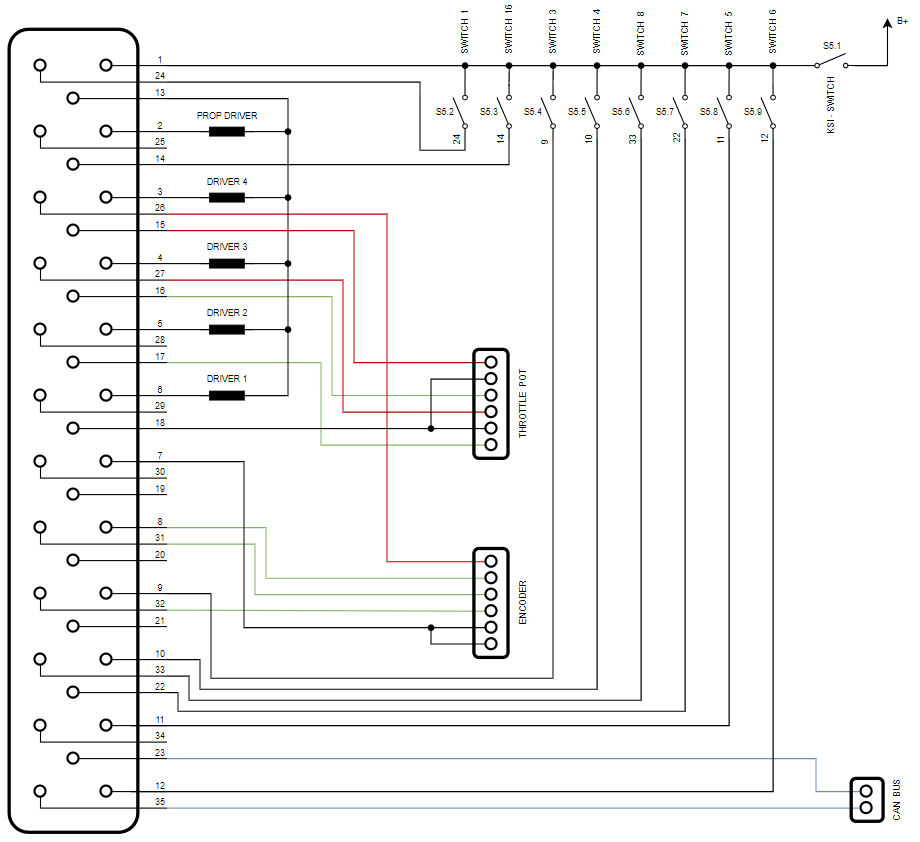
\includegraphics[scale=0.75]{figures/Antrieb/Antrieb_Steuerstromkreis.png}
		\caption{Grundaufbau des Steuerstromkreises}
	\end{center}
\end{figure}

\newpage

%% Digitale Eingänge (Digital Inputs) %%%%%%%%%%%%%%%%%%%%%%%%%%%%%%%%%%%%%%%%%%%%%%%
\subsubsection{Digitale Eingänge (Digital Inputs)}
Es gibt insgesamt 16 Pins, die als digitale Eingänge genutzt werden können, jedoch werden sieben Pins davon eigentlich als Ausgänge konfiguriert. 

\begin{figure}[H]
	\begin{center}
		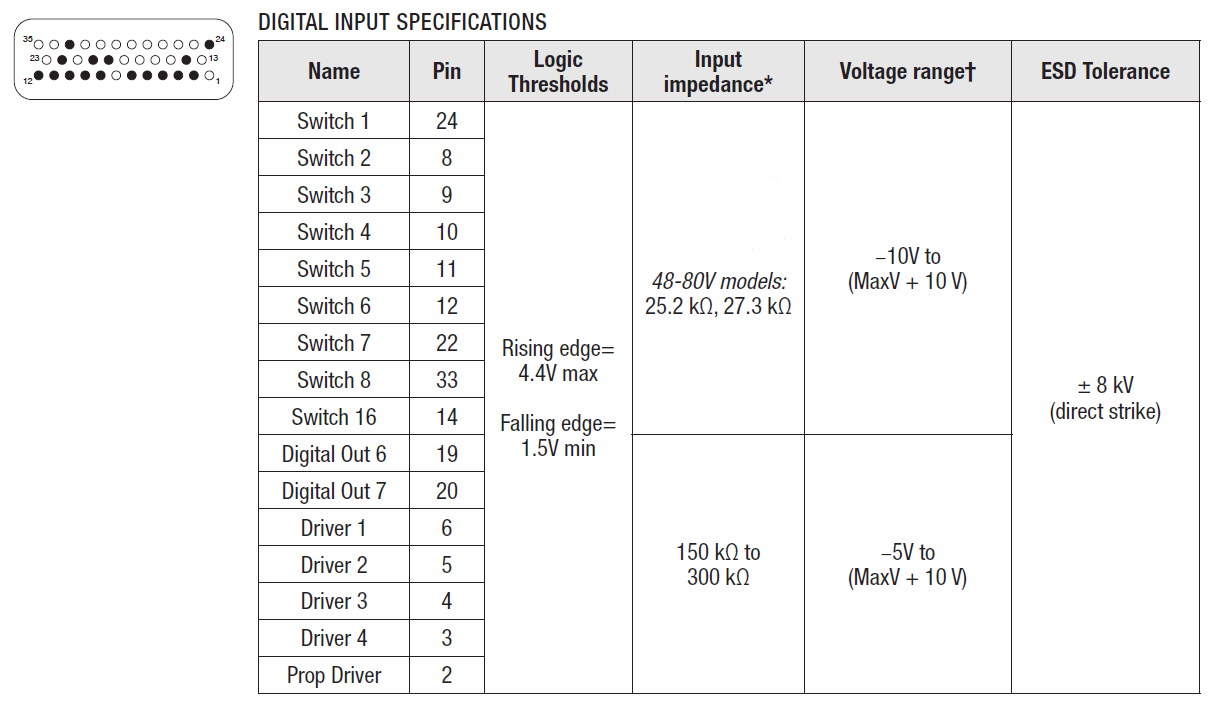
\includegraphics[width=\textwidth]{figures/antrieb/Digital_Input_Specifications.png}
		\caption{Digital Input Specifications}
	\end{center}
\end{figure}




%% Analoge Eingänge (Analog Inputs) %%%%%%%%%%%%%%%%%%%%%%%%%%%%%%%%%%%%%%%%%%%%%%%
\subsubsection{Analoge Eingänge (Analog Inputs)}
Es gibt insgesamt zwei Pins, die als analoge Eingänge verwendet werden können. Ein Pin davon wird jedoch im Normalfall für den Motortemperatur-Sensor verwendet. Die Eingänge, die für das Gas- und Bremspotentiometer verwendet werden, sind in dieser Kategorie nicht aufgelistet, obwohl diese ebenfalls als analoge Eingänge genutzt werden. Diese Pins sind jedoch speziell für die Gas- und Bremssteuerung konfiguriert und sollten im Normalfall auch dafür verwendet werden.

\begin{figure}[H]
	\begin{center}
		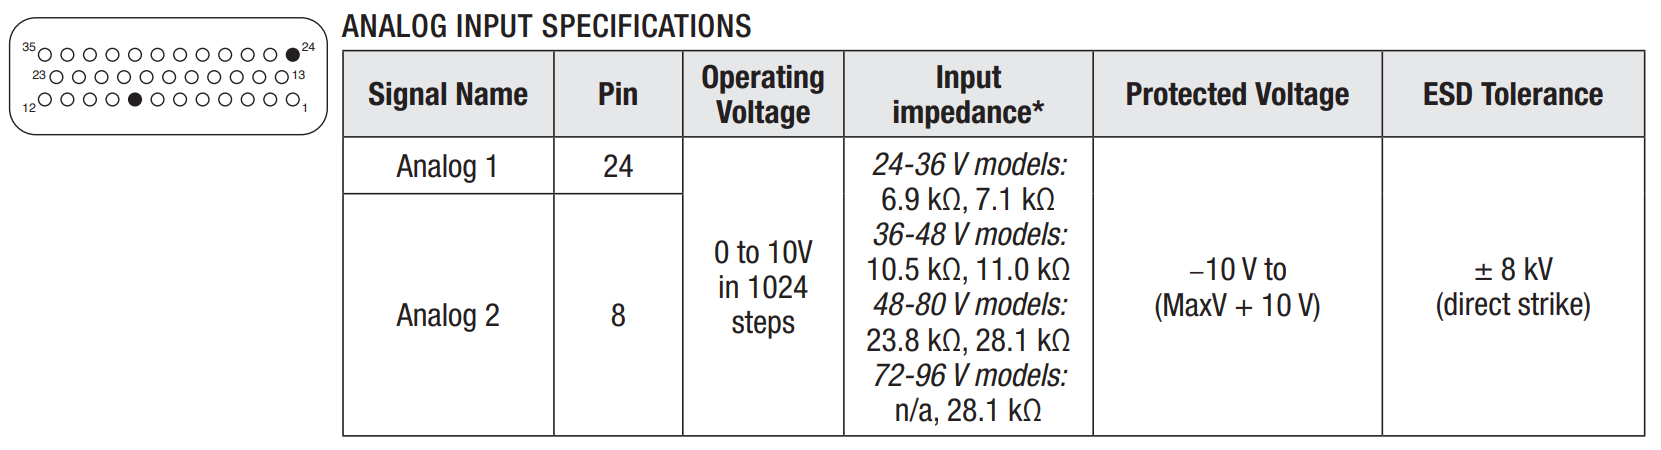
\includegraphics[width=\textwidth]{figures/antrieb/Analog_Input_Specifications.png}
		\caption{Analog Input Specifications}
	\end{center}
\end{figure}



\newpage



%% Gas- und Bremseingänge (Throttle and Brake Inputs) %%%%%%%%%%%%%%%%%%%%%%%%%%%%%%%%%%%%%%%%%%%%%%%
\subsubsection{Gas- und Bremseingänge (Throttle and Brake Inputs)}
Die zwei Gas- und Bremssteuerungs-Eingänge sind wegen der speziellen Auslegung von den analogen Eingängen abgegrenzt und können unabhängig voneinander programmiert werden. Sie sind optimiert für die Anwendung mittels Spannungssteuerung, 2-Draht Widerstandssteuerung oder 3-Draht Widerstandssteuerung. Bei der Spannungssteuerung benötigt man die Pins Pot Wiper und I/O Ground, bei der 2-Draht Widerstandssteuerung Pot Wiper und Pot Low und bei der 3-Draht Widerstandssteuerung Pot High, Pot Wiper und Pot Low. In unserem Fall benutzen wir beide Steuerungs-Eingänge für die 3-Draht Widerstandssteuerung, da der Gasdrehgriff über eine Drahtbrucherkennung verfügt. Das heißt, der Gasdrehgriff hat insgesamt zwei unabhängige 3-Draht Potentiometer-Ausgänge, welche beide für den Gaseingang benutzt werden.

\begin{figure}[H]
	\begin{center}
		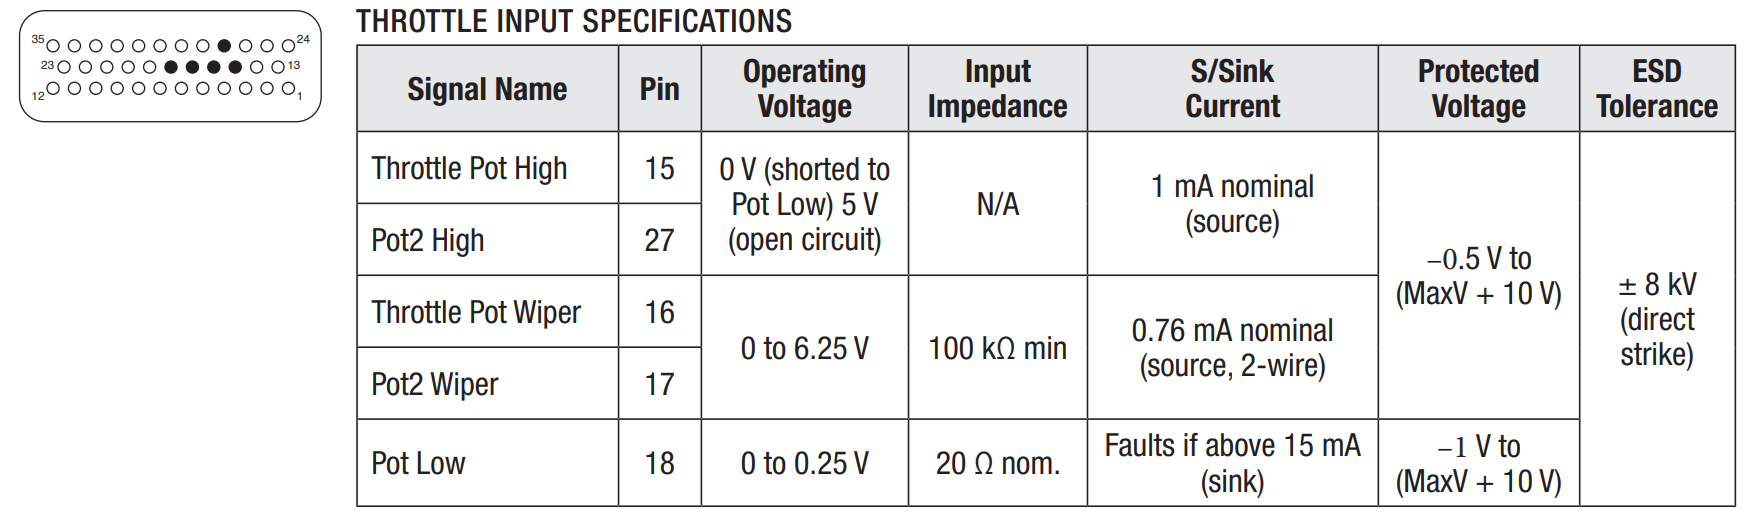
\includegraphics[width=\textwidth]{figures/antrieb/Throttle_Input_Specifications.png}
		\caption{Throttle Input Specifications}
	\end{center}
\end{figure}



%% Positionsrückmeldung vom Encoder (Position-feedback Input) %%%%%%%%%%%%%%%%%%%%%%%%%%%%%%%%%%%%%%%%%%
\subsubsection{Positionsrückmeldung vom Encoder (Position-Feedback Input)}
Diese zwei Pins sind intern dafür konfiguriert, die aktuelle Position der Motorwelle einzulesen, um eine optimale feldorienterte Ansteuerung des Motors durchführen zu können. Dabei gibt es die Möglichkeiten über einen Quadratur-Encoder oder einen Sin/Cos-Encoder. Da im Ashwoods-Motor ein Sin/Cos-Sensor verbaut ist, wurde dies vorab beim Motorcontroller eingestellt.

\begin{figure}[H]
	\begin{center}
		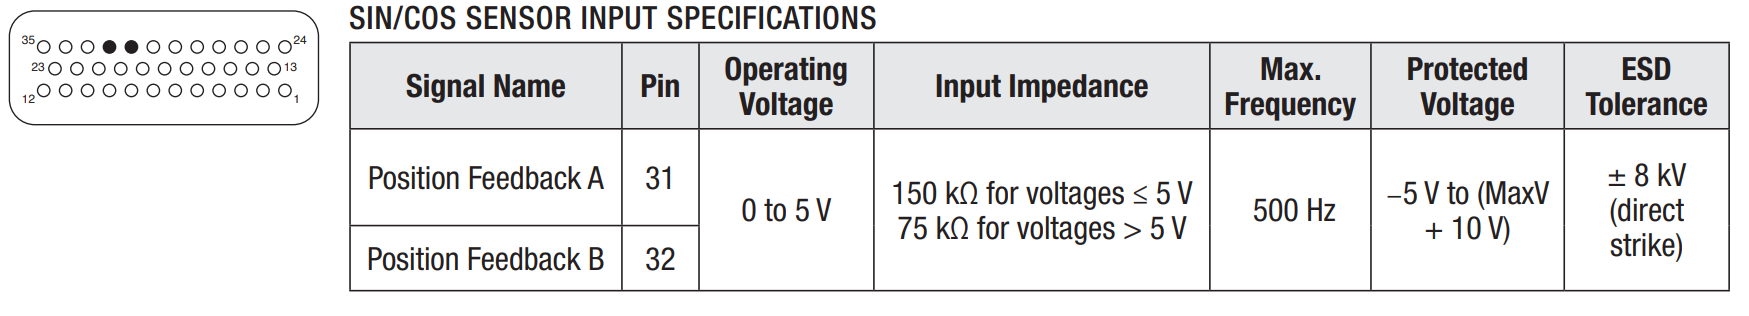
\includegraphics[width=\textwidth]{figures/antrieb/SinCosSensor_Input_Specifications.png}
		\caption{Sin/Cos Sensor Input Specifications}
	\end{center}
\end{figure}


\newpage


%% Prozessorversorgung und Spulenrücklauf (KSI and Coil Return) %%%%%%%%%%%%%%%%%%%%%%%%%%%%%%%%%%%%%%
\subsubsection{Prozessorversorgung und Spulenrücklauf (KSI and Coil Return)}
Der KSI-Eingang stellt die elektrische Versorgung aller Niederleistungs-Schaltkreise zur Verfügung. Dies  beinhaltet ebenfalls die Versorgung aller Ausgänge und die Kondensator-Vorlade-Funktion, welche dazu dient, die Kondensatoren über einen Widerstand vorzuladen, um hohe Einschaltströme zu verhindern. Der Spulenrücklauf stellt die Versorgung der pulsweitenmodulierbaren Ausgänge zur Verfügung und hat die gleiche Spannung wie der KSI-Pin. Die elektrische Trennung von KSI und Coil Return muss aufrechterhalten werden, um einen Verpolungsschutz gewährleisten zu können. 

\begin{figure}[H]
	\begin{center}
		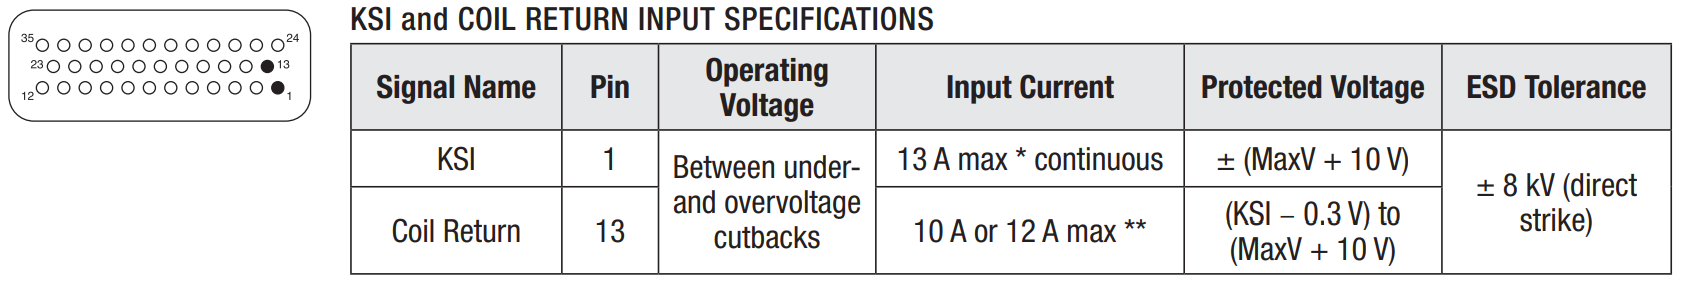
\includegraphics[width=\textwidth]{figures/antrieb/KSI_CoilReturn_Input_Specifications.png}
		\caption{KSI and Coil Return Input Specifications}
	\end{center}
\end{figure}



%% Analoge Ausgänge (Analog Outputs %%%%%%%%%%%%%%%%%%%%%%%%%%%%%%%%%%%%%%%%%%%%%%%
\subsubsection{Analoge Ausgänge (Analog Outputs)}
Der analoge Ausgang kann ein Spannungssignal von 0 bis 10V ausgeben. Dieser Ausgang ist für die Ausgabe über Anzeigeinstrumente, wie zum Beispiel eine Anzeige über den aktuellen Ladestand des Akkumulators, vorgesehen.

\begin{figure}[H]
	\begin{center}
		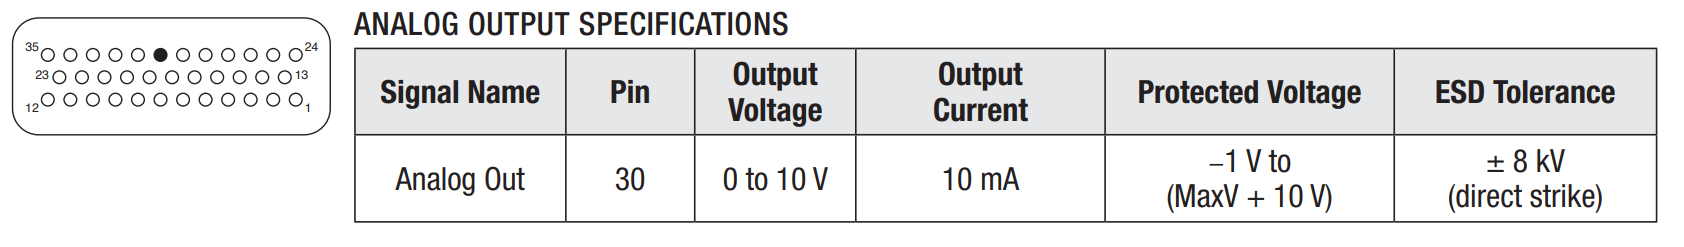
\includegraphics[width=\textwidth]{figures/antrieb/Analog_Output_Specifications.png}
		\caption{Analog Output Specifications}
	\end{center}
\end{figure}


\newpage



%% Digitale und Pulsweitenmodulierbare Ausgänge (Digital and PWM Outputs) %%%%%%%%%%%%%%%%%%%%%%%%%%%%
\subsubsection{Digitale und Pulsweitenmodulierbare Ausgänge (Digital and PWM Outputs)}
Es gibt insgesamt 7 digitale Ausgänge, wovon jedoch nur 5 für eine Pulsweitenmodulation konfiguriert werden können. Diese Ausgänge sind für induktive Lasten, wie zum Beispiel den Hauptschütz oder eine elektromagnetische Bremse, vorgesehen. Rein ohmsche Lasten können ebenfalls gesteuert werden, jedoch darf der zulässige Spitzenstrom nicht überschritten werden. Der Proportional-Driver kann bei richtiger Konfiguration auch für die Anzeige eines Tachometers hergenommen werden. Generell kann jeder Pin dieser Gruppe ebenfalls als digitaler Eingang benutzt werden.

\begin{figure}[H]
	\begin{center}
		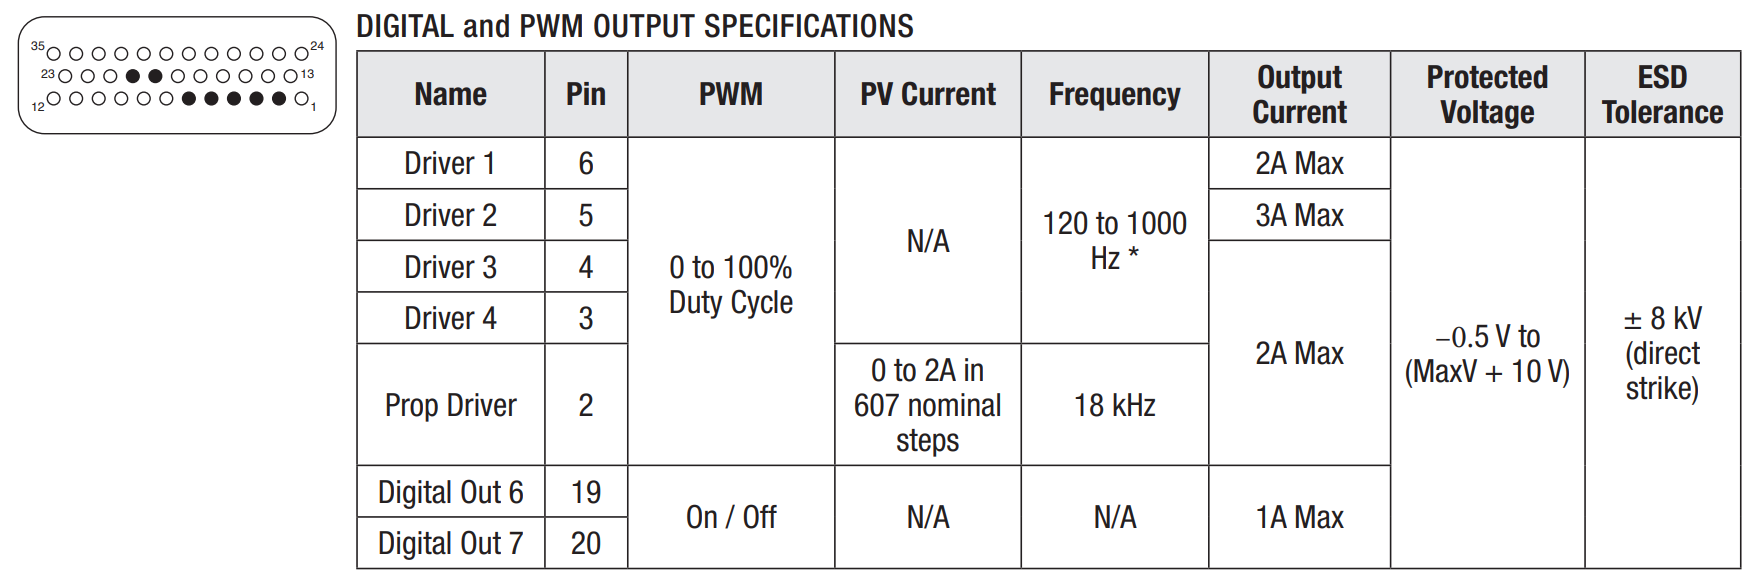
\includegraphics[width=\textwidth]{figures/antrieb/Digital_PWM_Output_Specifications.png}
		\caption{Digital and PWM Output Specifications}
	\end{center}
\end{figure}



%% Spannungsversorgungs-Ausgänge (Power Supply Outputs) %%%%%%%%%%%%%%%%%%%%%%%%%%%%%%%%%%%%%%%%%%%%%%
\subsubsection{Spannungsversorgungs-Ausgänge (Power Supply Outputs)}
Um kleine Schaltkreise, wie zum Beispiel einen LED-Indikator oder die Positionsrückmeldung des Encoders, mit Spannung versorgen zu können, gibt es zwei dafür vorgesehene Spannungsversorgungs-Ausgänge mit je einem Pin für 5V und 12V. Für diese Anwendungen gibt es ebenfalls noch einen Rücklauf, der als I/O Ground definiert wurde.

\begin{figure}[H]
	\begin{center}
		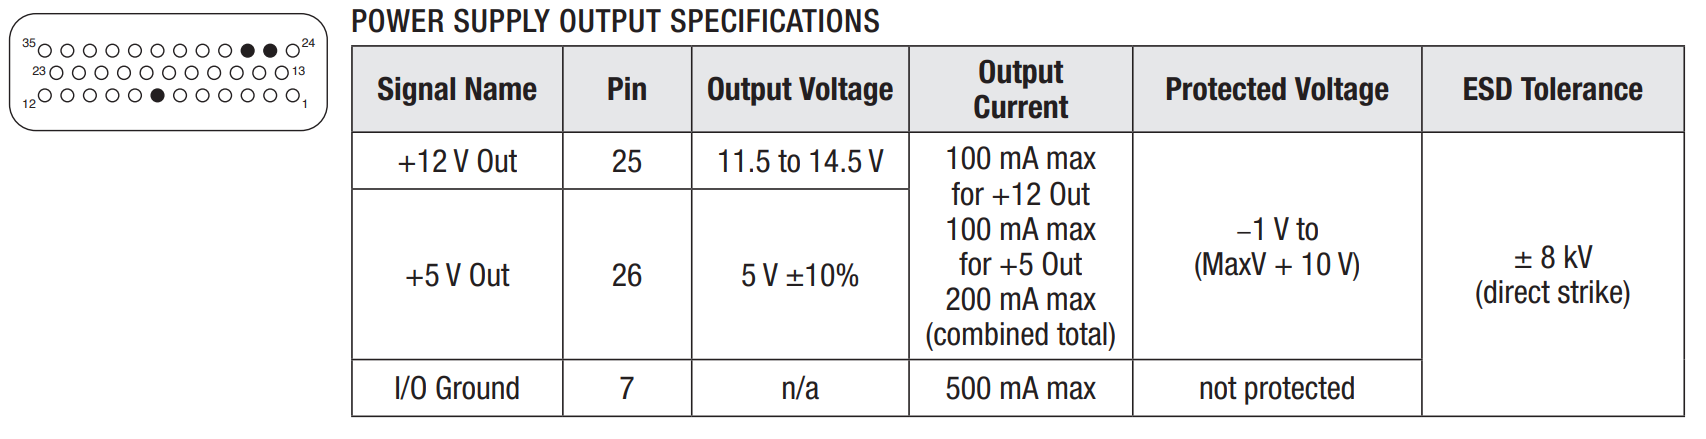
\includegraphics[width=\textwidth]{figures/antrieb/Power_Supply_Output_Specifications.png}
		\caption{Power Supply Output Specifications}
	\end{center}
\end{figure}


\newpage


%% Kommunikations-Ports %%%%%%%%%%%%%%%%%%%%%%%%%%%%%%%%%%%%%%%%%%%%%%%
\subsubsection{Kommunikations-Ports}
Für die Kommunikation mit anderen Betriebsmitteln stellt uns der Motorcontroller zwei Möglichkeiten zur Verfügung, den CAN-Bus und die serielle Schnittstelle. Da sich unser Projektteam auf die Nutzung des CAN-Busses geeinigt hat, wird die serielle Schnittstelle nicht verwendet. Die zwei Pins CAN Term High und CAN Term Low werden ebenfalls nicht benötigt, denn diese dienen nur dazu, den CAN-Bus vorübergehend funktionsunfähig zu schalten. Programmtechnisch gibt es drei Möglichkeiten zur Konfiguration des CAN-Busses, dies wird jedoch im Punkt Software genauer erklärt.

\begin{figure}[H]
	\begin{center}
		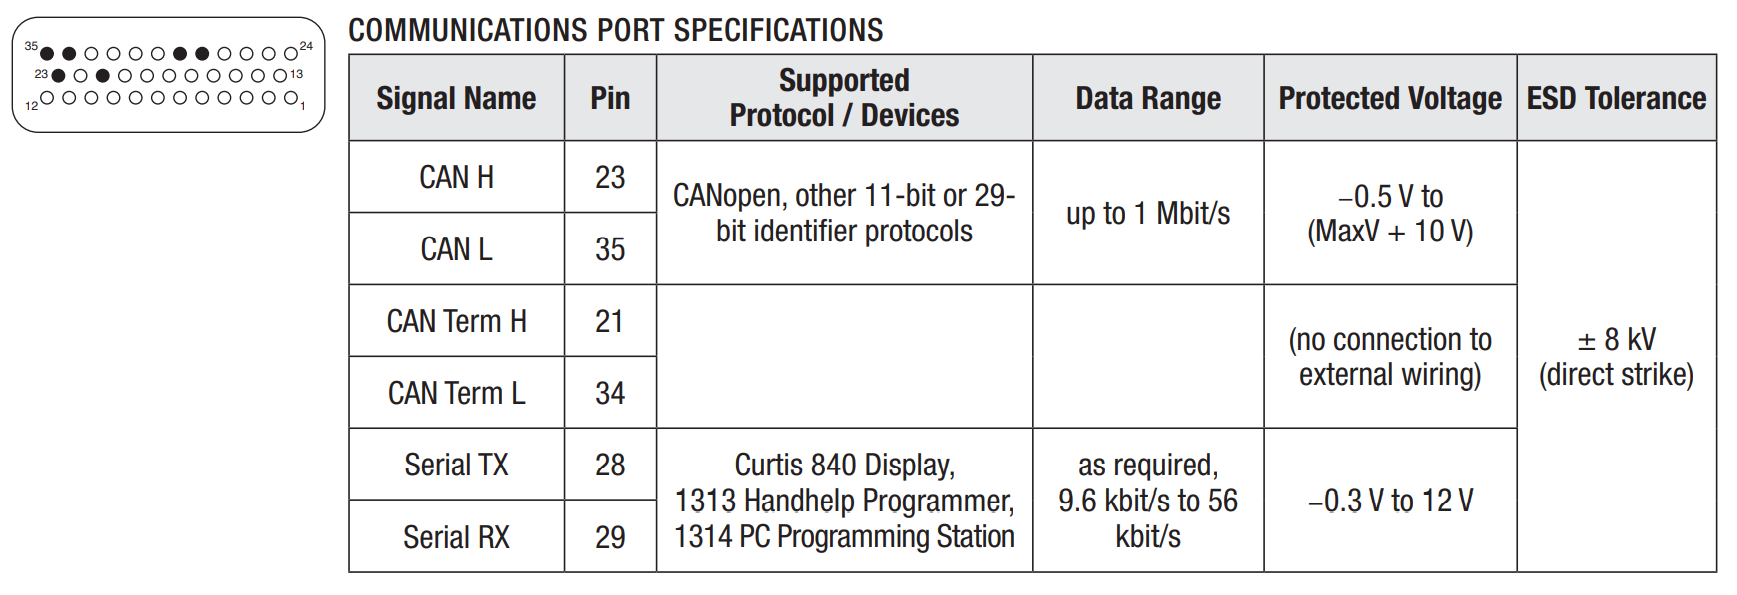
\includegraphics[width=\textwidth]{figures/antrieb/Communications_Port_Specifications.png}
		\caption{Communications Port Specifications}
	\end{center}
\end{figure}



\newpage


%% Softwareaufbau %%%%%%%%%%%%%%%%%%%%%%%%%%%%%%%%%%%%%%%
\section{Softwareaufbau des Antriebssystems}
Der Softwareaufbau des Antriebssystems kann grob in 3 Grundfunktionen unterteilt werden:
\\[5mm]
\begin{itemize}
	\item \textbf{Parameterbasierte Programmierung (Programmer)}
	\\ \medskip Umfasst alle Parameter und die vornehmbaren Konfigurationsmöglichkeiten.
	\medskip
	\item \textbf{Drehmomentsteuerung (Torquecontrol)}
	\\ \medskip Beinhaltet alle Parametereinstellungen, welche für die Drehmomentsteuerung ausschlaggebend sind.
	\medskip
	\item \textbf{Vehicle-Control-Language (VCL) Programmierung}
	\\ \medskip Umfasst das gesamte Programm, welches mit der Vehicle-Control-Language realisiert wurde.
	\\ Ein Großteil dieses Programms beschäftigt sich hierbei mit der Kommunikation zwischen der Motorsteuerung und dem Raspberry PI.
\end{itemize}

\newpage

%% Steuerung der In- und Outputs %%%%%%%%%%%%%%%%%%%%%%%%%%%%%%%%%%%%%%%%%%%%
\subsection{Parameterbasierte Programmierung (Programmer)}
\subsubsection{Allgemeines}
In dem Curtis Integrated Toolkit befindet sich unter anderem die Funktion \glqq Programmer\grqq{}, welche sehr viele Applikationseinstellungen für die Controllerprogrammierung zur Verfügung stellt. Es gibt mehrere verschiedene Menüs, welche die jeweils zugehörigen Parametergruppen auflisten. Viele Variablen können konfiguriert werden, andere werden nur für die Ausgabe aktueller Werte wie zum Beispiel die aktuelle Geschwindigkeit oder Temperatur verwendet. Die Parameter können je nach Anwendung und Funktion verschiedene Einheiten und einstellbare Wertebereiche besitzen. Sehr vorteilhaft sind hierbei die meist vorhandenen Kurzbeschreibungen im Curtis Integrated Toolkit oder die Parameterdeklaration in der Anleitung.

\subsubsection{Funktionen}
\textbf{Throttle and Brake}\\[1mm]
Die Hauptfunktion dieser Parametergruppen ist die genaue Einstellung der Potentiometer-Eingänge für den Bremsvorgang, Vorwärts- und Rückwärtsbetrieb. Es können der Start- und Endwert des Potentiometer festgelegt werden, ebenso bestimmte Formänderungen der Eingangskurve, welche die Intensität des Gas- bzw. Bremsbefehls abhängig von der Potentiometerstellung beschreibt. Ebenso gibt es mehrere mögliche Sicherheitskonfigurationen, Filtereinstellungen und auch die Möglichkeit der Ansteuerung mittels VCL.\\[3mm]

\textbf{CAN Interface}\\[1mm]
Das CAN-Interface wird in unerer Anwendung nicht benötigt, denn die Kommunikation wurde mittels VCL-CAN umgesetzt. Die vorgefertigte Version CANopen bietet jedoch auch mehrere Einstellungsmöglichkeiten, wie ID und Taktfrequenzanpassungen. Ebenfalls gibt es jeweils 4 Datenpakete, welche für den Senden- und Empfangenvorgang konfiguriert werden können.
\\[3mm]

\textbf{Battery Setup}\\[1mm]
In diesem Parametermenü kann die Nennspannung festgelegt werden, ebenfalls gibt es mehrere Einstellungsmöglichkeiten, welche in einem Über- oder Unterspannungsfall von Bedeutung sind. Um den Ladestand des Akkumulators besser abschätzen zu können, sollten hier auch bestimmte Eigenschaften festgelegt werden.
\\[3mm]

\textbf{Main Contactor}\\[1mm]
Dieses Menü dient zur Konfiguration Hauptschütz (Hochleistungs-Relais). Die Ansteuerungsspannung wird hier genau beschrieben, nach dem Schließen des Schützes kann eine kleiner Spannung zum halten der Kontakte verwendet werden. Ebenfalls kann eine Zeitverzögerung eingestellt werden, welche bestimmt wie lange der KSI-Pin geöffnet sein darf, bevor der Hauptschütz geöffnet wird. Diese Funktion kann sehr wichtig sein, denn ein Wechsel des Antriebsmodus kann somit ebenfalls während des Betriebs erfolgen (Gaseingang muss aber 0\% sein).
\\[3mm]

\textbf{Pump Contactor}\\[1mm]
.
\\[3mm]

\textbf{EM Brake Control}\\[1mm]
.
\\[3mm]

\textbf{Emergency Reverse (EMR)}\\[1mm]
.
\\[3mm]

\textbf{Interlock Braking}\\[1mm]
.
\\[3mm]

\textbf{Dual Drive}\\[1mm]
.
\\[3mm]

\textbf{Vehicle und Supervision}\\[1mm]
.
\\[3mm]

\textbf{Current Limits}\\[1mm]



\newpage

%% Drehmomentsteuerung %%%%%%%%%%%%%%%%%%%%%%%%%%%%%%%%%%%%%%%%%%%%
\subsection{Drehmomentsteuerung (Torquecontrol)}
Die Drehmomensteuerung wird mithilfe von 12 unterschiedlichen Parametern beschrieben. Generell können diese Parameter eher als Feineinstellungen angesehen werden, da der grundsätzliche Vorgang immer der gleiche bleibt. Mit diesen Parametern werden jedoch die maximale Geschwindigkeit, die Reaktionszeit und die Aggresivität des Motors genau definiert, um das gewünschte Beschleunigungsmuster erhalten zu können.

\vspace{1mm}
 
\subsubsection{Parameter}
Grundsätzlich lassen sich diese Parameter in zwei Hauptgruppen unterscheiden:
\\[5mm]
\begin{itemize}
	\item \textbf{Geschwindigkeitsbegrenzer-Parameter (Speed-Limiter)}
	\\ \medskip Bestimmen die maximale Geschwindigkeit und die Begrenzungsparameter des KPI-Reglers.
	\medskip
	\item \textbf{Reaktions-Parameter (Response)}
	\\ \medskip Bestimmen die verschiedensten Ansprechzeiten und Drehzahlen für bestimmte Ereignisse.
\end{itemize}

\vspace{5mm}

Diese Parameter werden in den folgenden Tabellen noch genau erklärt. Für ein besseres Verständnis können ebenfalls die englischen Tabellen \glqq SPEED LIMITER MENU\grqq{} und \glqq RESPONSE MENU\grqq{}, aber auch die zugehörigen Abbildungen \glqq Figure 9-11\grqq{} aus der Anleitung herangezogen werden.




\begin{table}[H]
	\begin{tabular}{|lcp{8cm}|}\hline
	\rowcolor[gray]{0.8}\textbf{Parameter} & \textbf{Einstellungsbereich} &\textbf{Beschreibung}\\[3pt]
		Max Speed & 500 - 8000 U/min & Definiert die maximale Geschwindigkeit in U/min,\\
		Max\_Speed\_TrqM & 500 - 8000	& welche mittels der Drehmomentsteuerung\\&& angesteuert werden kann. (Unabhängig von der Gasdrehgriff-Stellung)\\\hline
		Kp 	& 0 – 100 \% 	& Legt fest, wie aggressiv der Drehzahlregler versucht,\\
		Kp\_TrqM	& 0 – 8192			& die Motordrehzahl auf die maximale Drehzahl zu begrenzen. Größere Werte sorgen für eine genauere Kontrolle, können jedoch zu Schwankungen führen. Bei einem zu niedrigen Kp kann die maximal\\&& Geschwindigkeit den Parameter Max Speed\\&& überschreiten.\\\hline
		Ki 			& 5 – 100 \% 		& Mit diesem Parameter kann die Integralregelung\\
		Ki\_TrqM	& 50 – 1000 		& genauer beschrieben werden, welche die Drehzahl-begrenzung unterschiedlich stark beeinflusst, abhängig von der aktuellen Regelabweichung. Größere Werte ermöglichen eine schnellere Regelung, können jedoch zu Schwankungen führen. Bei zu niedrigen Werten kann es lange dauern, bis sich der Motor bei einer Überdrehzahl dem Max Speed nähert. \\\hline
		Kd    		& 0 – 100 \% 	& Beschreibt die Dämpfung, wenn sich das Fahrzeug\\
		Kd\_TrqM	& 0 – 8192	 	& der Höchstgeschwindigkeit nähert, dadurch werden Überschwingungen verringert. Bei einem zu hohen Kd kann es lange dauern, bis die Höchstgeschwindigkeit erreicht wird. Wenn Kd zu niedrig eingestellt ist, kann die Höchstgeschwindigkeit überschritten\\&& werden, insbesondere beim bergab Fahren. \\\hline	
	\end{tabular}	
	\caption{Geschwindigkeitsbegrenzer-Parameter}
	\label{tab:Geschwindigkeitsbegrenzer-Parameter}
\end{table}

\newpage

\begin{table}[H]
	\begin{tabular}{|lcp{6cm}|}\hline
	\rowcolor[gray]{0.8}\textbf{Parameter} & \textbf{Einstellungsbereich} &\textbf{Beschreibung}\\[3pt]
		Accel Rate 	& 0.1 - 30.0 s 		& Legt fest, wie lange es dauert, bis das\\
		Accel\_Rate\_TrqM & 100 - 30000	& Motordrehmoment bei Vollgas auf das Maximum angestiegen ist. Größere Werte bedeuten eine langsamere\\&& Reaktion. \\\hline
		Accel Release Rate	& 0.1 - 2.0 s 		& Legt fest, wie schnell die Verzögerung\\
		Accel\_Release\_Rate\_TrqM & 100 - 2000 & des Fahrzeugs bei einem loslassen des Gasdrehgriffs eingeleitet wird. Bei\\&& einem geringen Wert wird der Übergang abrupt eingeleitet. Ist der Wert zu hoch eingestellt, fährt das Fahrzeug für kurze Zeit weiter.\\\hline
		Brake Rate 	& 0.1 - 5.0 s 		& Legt fest, wie lange es dauert, bis das\\
		Brake\_Rate\_TrqM & 100 - 5000	& Bremsmoment bei einem startenden Bremsvorgang oder einem Fahrt-richtungswechsel aufgebaut wird. Größere Werte bedeuten einen\\&& schonenderen Bremsvorgang. \\\hline
		Brake Release Rate	& 0.1 - 2.0 s 		& Beschreibt, wie schnell sich das Brems-\\
		Brake\_Release\_Rate\_TrqM & 100 - 2000	& moment löst, wenn das Fahrzeug vom Bremsvorgang zum Fahrbetrieb\\&& wechselt. Bei zu hohen Werten wird der Bremsvorgang noch kurzzeitig\\&& fortgeführt.  \\\hline
		Neutral Braking    & 0 – 100 \% 	& Der neutrale Bremsvorgang tritt auf,\\
		Neutral\_Braking\_TrqM & 0 - 32767 	& wenn der Gasdrehgriff losgelassn wird oder keine Fahrtrichtung gewählt\\&& wurde. Der neutrale Bremsparameter ist von 0 bis 100\% des maximalen\\&& Rekuperationsstromes einstellbar. \\\hline
		Neutral Taper Speed	& 200 - 6000 U/min 	 & Legt die Motordrehzahl fest, an welcher\\
		Neutral\_Taper\_Speed\_TrqM & 200 - 6000 & der neutrale Bremsstrom rückgespeist wird, wenn der Gasdrehgriff losgelassen wird. Bei einem zu geringen Wert kann es zu Schwankungen kommen.\\\hline
		Forward Full Restraint Speed & 100 – 32000 U/min & Legt den Geschwindigkeitspunkt fest,\\   Forward\_Full\_Restraint\_Speed\_TrqM & 100 - 32000 & an dem der volle Rekuperationsstrom rückgespeist wird, um das Vorwärts-rollen des Fahrzeugs zu verhindern. Kann auch als Parameter für die              \\&&Rückhaltestärke angesehen werden.\\&& Bei einem zu geringen Wert kann es zu Schwankungen kommen.  \\\hline
		Back Full Restraint Speed & 100 – 32000 U/min & Legt den Geschwindigkeitspunkt fest,\\ 		Back\_Full\_Restraint\_Speed\_TrqM & 100 – 32000 & an dem der volle Rekuperationsstrom rückgespeist wird, um das Rückwärts-rollen des Fahrzeugs zu verhindern. Kann auch als Parameter für die 				\\&&Rückhaltestärke angesehen werden.\\&& Bei einem zu geringen Wert kann es zu Schwankungen kommen. \\\hline		
	\end{tabular}	
	\caption{Reaktions-Parameter}
	\label{tab:Reaktions-Parameter}
\end{table}


\newpage

\subsubsection{ECO- und Sportmodus (Speed-Mode-Select)}
Die oben genannten Parameter werden für die Erstellung der unterschiedlichen Antriebsmodi verwendet. Für den Ecomodus werden für die Parameter höhere Reaktionszeiten und weniger Aggressivität gewählt, daraus ergibt sich ein gemütlicherer und schonenderer Fahrbetrieb, welcher gleichzeitig weniger Leistung verbraucht. Für den Sportmodus hingegen werden kürzere Reaktionszeiten und höhere Aggressivität gewählt, daraus ergibt sich ein sportlicheres Fahrverhalten, die gewünschte Geschwindigkeit wird schneller erreicht. Natürlich zieht dieser Antriebsmodus einen erhöhten Leistungsverbrauch nach sich. Der Wechsel des Antriebsmodus bedeutet jedoch eine Veränderung kritischer Parameter, weshalb der KSI-Pin aus- und eingeschalten werden muss, um den normalen Fahrbetrieb wieder aufnehmen zu können. Da jedoch ein ausschalten des KSI-Pins zum sofortigen Stillstand (Einleiten des Bremsvorgangs bis die Geschwindigkeit 0 ist) des Motorrades führt, kann der Wechsel des Antriebsmodus nur im Stillstand erfolgen. Die einzelnen Modi können beliebig konfiguriert werden und auch im Nachhinein mittels dem Curtis Integrated Toolkit bzw. VCL-Studio sehr schnell und leicht verändert oder angepasst werden. Vorerst wird es nur zwei unterschiedliche Antriebsmodi geben, da in diesem Fall nur ein Pin für die Selektierung benötigt wird (1 digitaler Eingang). Wenn in Zukunft jedoch weiterhin Interesse an weiteren unterschiedlichen Antriebsmodi besteht, können diese mit relativ wenig Aufwand hinzugefügt werden.

\vspace{5mm}

Hier eine Tabelle der einzelnen Parameter im ECO- und im Sportmodus:

\vspace{2mm}

\begin{table}[H]
	\begin{tabular}{|l>{\centering\arraybackslash}p{4.5cm}>{\centering\arraybackslash}p{4.5cm}|}\hline
	\rowcolor[gray]{0.8}\textbf{Parameter} & \textbf{ECO-Modus} &\textbf{SPORT-Modus}\\[3pt]
		Max Speed 						& 7000 U/min	& 8000 U/min 	\\\hline
		Kp 								& 30 \% 		& 40 \% 	 	\\\hline
		Ki 								& 30 \% 		& 40 \% 	 	\\\hline
		Kd    							& 15 \% 		& 10 \%		 	\\\hline		
		Accel Rate 						& 2 s 			& 1 s		 	\\\hline
		Accel Release Rate				& 1 s 	 		& 0.4 s		 	\\\hline
		Brake Rate 						& 2 s 	 		& 1 s		 	\\\hline
		Brake Release Rate				& 1 s 	 		& 0.4 s		 	\\\hline
		Neutral Braking    				& 15 \% 		& 10 \%		 	\\\hline
		Neutral Taper Speed    			& 500 U/min 	& 800 U/min 	\\\hline
		Forward Full Restraint Speed	& 800 U/min 	& 500 U/min		\\\hline
		Back Full Restraint Speed    	& 800 U/min 	& 500 U/min		\\\hline		
	\end{tabular}	
	\caption{Antriebsmodi}
	\label{tab:Antriebsmodi}
\end{table}

\vspace{2mm}

\textbf{Konventionelle Umsetzung} \\
\vspace{2mm}
In konventionellen E-Motorrädern wird bei der Auswahl zwischen den Antriebsmodi ECO-Normal-Sport eine 7-Punkte Map hinterlegt, welche die Drehzahl abhängig vom Drehmoment beschreibt. Da dies für die schulische Umsetzung aber ebenfalls zu zeitintensiv wäre, wird dies wahrscheinlich bei späteren Optimierungen hinzugefügt.


 

\newpage




%% Kommunikation %%%%%%%%%%%%%%%%%%%%%%%%%%%%%%%%%%%%%%%%
\subsection{Vehicle-Control-Language (VCL) Programmierung}
\subsubsection{Grundfunktion}
Die Vehicle-Control-Language ist ein eigener Abschnitt der Programmierung und von der Grundidee auch sehr unterschiedlich. Die normale Parameterprogrammierung vereinfacht die generelle Programmierung des Curtis Controllers zwar sehr, beschränkt die Anzahl der Möglichkeiten jedoch auf die Anzahl der Parameter und deren Konfigurationsmöglichkeiten. Die VCL-Programmiersprache bietet hierbei eine sehr gute Erweiterungsmöglichkeit und bei Kombination der beiden Programmierarten kann die Programmierung des Curtis Controllers optimiert und enorm erweitert werden. Die Vehicle-Control-Language ist eine Programmiersprache auf der Basis von C und das VCL-Studio sieht der Benutzeroberfläche eines normalen Programms mit integriertem Editor und Compiler, wie zum Beispiel Dev-C++, sehr ähnlich. Da in diesem Fall jedoch jeder beliebige Programmcode verfasst werden kann, bietet VCL nahezu endlose Möglichkeiten. Die wichtigsten Grundlagen, auf die man bei der Programmierung von VCL aufpassen muss, sind in den beigelegten Skripten \glqq WIN VCL User's Guide\grqq{}, \glqq VCL Programmer's Guide\grqq{} und \glqq VCL Common Functions\grqq{} im Anhang genauer erklärt. Das Wichtigste ist jedoch die Kenntnis darüber, dass mit dem VCL-Studio nicht nur die vorhandenen oder selbsterstellten VCL-Variablen verändert werden können. Die meisten Variablen, die in den Parametermenüs vorhanden sind, können ebenfalls eingelesen und beschrieben werden. Hier ist natürlich Vorsicht geboten, denn viele Parameter dürfen in keinem Fall während des Betriebs geändert werden. Bei wichtigen Variablen muss daher auch ein Aus- und Einschalten des KSI-Pins durchgeführt werden, um die Veränderung wirksam zu machen und Komplikationen zu vermeiden. Generell ist die Hauptaufgabe einer ausgefeilten VCL-Programmierung jedoch die Automatisierung des gesamten E-Motorrades. Zum Beispiel kann beim Auftritt eines Fehlers automatisch ein zugehöriger Fehlerbehebungsvorgang eingeleitet werden. Da wir in unserem Projekt jedoch nur ein sehr kleines Zeitfenster zur Verfügung haben, konnte das VCL-Programm nicht derartig ausgereift werden. In unserem Fall beschränkt sich die VCL-Programmierung fast ausschließlich auf die Kommunikation mit dem Raspberry PI, denn die Lösung über VCL-CAN schien uns einfacher und vorallem viel flexibler wie die vorgefertigte Programmierung \glqq CANopen\grqq{} zu verwenden. 

\newpage

\subsubsection{Kommunikation (CAN-Bus)}
Die Kommunikation erfolgt grundsätzlich nur in eine Richtung, da dies nicht nur einfacher zu realisieren war, sondern für unsere Anwendungen auch völlig ausreicht. Der Curtis Controller sendet die ausgewählten Parameter immer in der selben Reihenfolge an den Raspberry PI, dafür wurden 3 unterschiedliche Datenpakete mit jeweils einem einzigartigen Identifier und 7 folgenden Parametern erstellt. Ein Parameter enthält immer 4 Hexadezimalzahlen, also insgesamt 2 Byte. Wenn ein Fehler am Motorcontroller erkannt wurde, wird nach dem dritten Datenpaket noch ein zusätzliches Fehler-Datenpaket eingeschoben. Wenn zum Beispiel zwei Fehler am Controller vorliegen, werden diese 2 Fehler nach dem Fehler-Identifier (FFFF) gesendet, danach werden die 5 weiteren freien Plätze des Fehler-Datenpakets mit dem Fehler-Identifier aufgefüllt. Nachdem das Fehler-Datenpaket gesendet wurde, werden die ersten 7 Fehler vom Datenspeicher gelöscht, liegt der Fehler jedoch weiterhin vor, kann dieser auch nicht gelöscht werden. Hier werden die Datenpaket mit den zugehörgen Parametern noch ausführlich dargestellt:

\setlength{\tabcolsep}{9pt}
\begin{table}[H]
	\begin{tabular}{|lcc>{\centering\arraybackslash}p{5cm}|}\hline
	\rowcolor[gray]{0.8} & \textbf{Datenpaket 1} & \textbf{Datenpaket 2} & \textbf{Datenpaket 3}\\[3pt]
		Identifier	& FFFC & FFFD & FFFE\\\hline
		Parameter 1 & Vehicle\_Speed & Vehicle\_Speed & Vehicle\_Speed\\\hline
		Parameter 2 & Current\_RMS	& Capacitor\_Volts & Vehicle\_Acceleration\\\hline
		Parameter 3 & Controller\_Temperature & BDI\_Percentage & Vehicle\_Odometer\\\hline
		Parameter 4 & Motor\_Temperature	& Interlock	& Time\_to\_Capture\_Speed\_1\\\hline		
		Parameter 5	& Motor\_Power 	& Throttle\_Command & Time\_to\_Capture\_Distance\_1\\\hline
		Parameter 6	& Motor\_Torque 	& Brake\_Command	& Braking\_Distance\_Captured\\\hline
		Parameter 7 & Modulation\_Depth & EMR\_State & Distance\_Since\_Stop\\\hline		
	\end{tabular}	
	\caption{Datenpakete Deklaration}
	\label{tab:Datenpakete_Deklaration}
\end{table}

Der gesamte VCL-Programmcode befindet sich im Anhang, auffällig ist hierbei unter anderem die enorm lange Zeitverzögerung, welche den selben Delay-Befehl 3330 mal beinhaltet. Die gewünschte CAN-Bus Übertragungsfrequenz beträgt 100ms, da jedoch der integrierte Logic-Controller eine sehr viel kürzere applikationsabhängige Taktfrequenz besitzt, erwies sich das Aussenden von Parametern in der selben Reihenfolge vorerst als sehr schwierig. Es wurden viele unterschiedliche Methoden versucht, jedoch erwies sich die Synchronisation der beiden Taktfrequenzen als die einfachste. Da ebenfalls sehr wenig hilfreiche Informationen im Internet zu finden waren, wurde die Realisierung mit einer besseren Methode vernachlässigt. Die Vereinfachung bzw. Verkürzung der langen Zeitverzögerung mit einer Schleife oder ähnlichem erwies sich ebenfalls als schwierig und fehleranfällig, wurde deshalb weggelassen.

\newpage

\subsubsection{Speed-Mode-Select}
Die Speed-Mode-Select Programmierung gehört eigentlich auch zum Punkt Drehmomentsteuerung, dieses Programm wurde aber ebenfalls in der Vehicle-Control-Language realisiert. Die zugehörigen Parmeter, welche ausschlaggebend für die Drehmomentsteuerung sind, wurden bereits genau erklärt. Grundsätzlich ist das VCL-Programm sehr einfach und kurz aufgebaut, die Parameter zur Drehmomentsteuerung werden abhängig von einem digitalen Eingang verändert. Der digitale Eingang wird mittels eines externen Schalters realisiert, dieser wurde auf der Lenkstange befestigt. Wenn der Schalter auf den ECO-Antriebsmodus geschalten wurde, werden die Parameter für den ECO-Antriebsmodus an den Drehmomentregler weitergegeben. Bei der Auswahl des Sport-Antriebsmodus werden die Parameter für den Sport-Antriebsmodus an den Regler weitergegeben.\\ 
\vspace{5mm}
Wie im folgenden Programmschnippsel zu erkennen ist, ist der Aufbau dieses Programms äußerst einfach. Aufpassen muss man bei der Überschreibung der Parameter, da nicht die Werte mit den Einheiten, sondern die absoluten Werte verwendet werden müssen. Vorallem bei den Parametern des PID-Reglers sind unterschiedliche Absolutwerte vorgegeben, diese müssen auf den gewünschten Prozentwert scaliert werden.
\vspace{2mm}
\begin{figure}[H]
	\begin{center}
		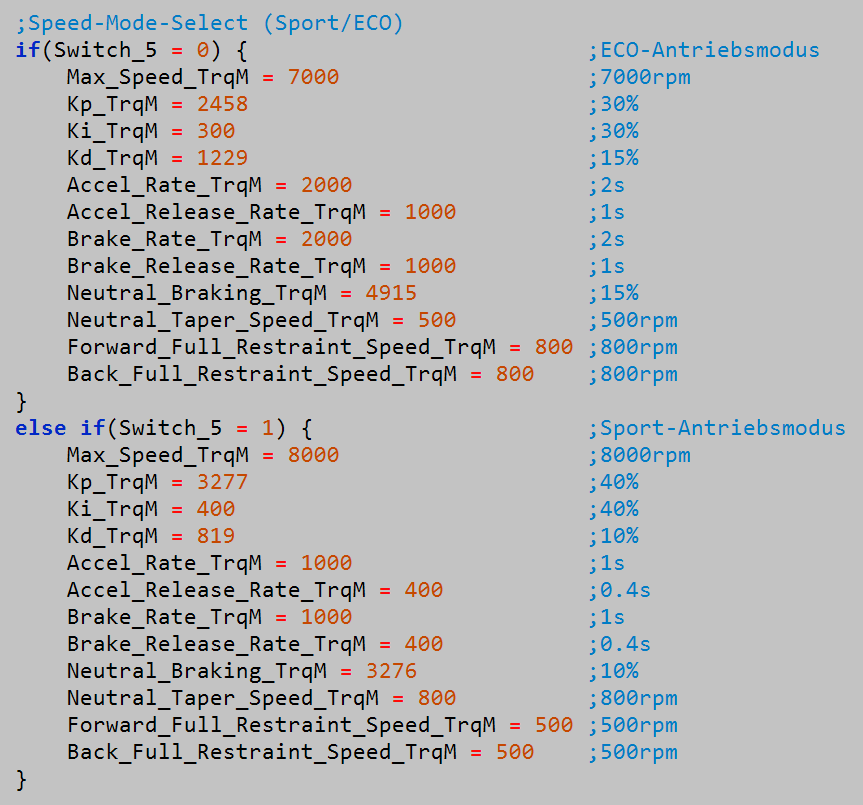
\includegraphics[scale=0.5]{figures/antrieb/ECO_Sport_Select_Programmschnippsel.png}
		\caption{ECO/Sport-Select Programmschnippsel}
	\end{center}
\end{figure}

\newpage


%% Inbetriebnahme %%%%%%%%%%%%%%%%%%%%%%%%%%%%%%%%%%%%%%%
\section{Inbetriebnahme}
\subsection{Leonard-Versuchsaufbau}
\textbf{Grundidee:}
\\[2mm]
Der Bau des Li-Ionen-Akkumulators hat sich leider sehr verzögert. Um effektiv an der Inbetriebnahme des Antriebssystems weiterarbeiten zu können, musste vorübergehend eine alterntive Spannungsversorgung gefunden werden, welche für die Anforderungen der Motorsteuerung geeignet ist. Da der Motor und die Motorsteuerung jedoch eine bipolare Spannungsquelle benötigen, um ordnungsgemäß in Betrieb genommen werden zu können, erwies sich dies vorerst schwierieger als gedacht. Die Beschaffung eines bipolaren Netzteils erwies sich als zu kosten- und zeitintensiv, weshalb der Betreuungslehrer vorschlug, die bipolare Spannungsquelle mittels eines Leonard-Umformers zu realisieren.
\\[5mm]

\textbf{Fazit:}
\\[2mm]
Der erste Schritt bei der Inbetriebnahme des Motors ist der Testlauf (Commissionierung) zur Ausmessung und Einstellung der Motorparameter. Bei der Durchführung dieses Testlaufs stoppte die Motorsteuerung jedoch immer wieder nach kurzer Zeit. Auch viele weitere Versuche bei geänderten Testparametern oder zusätzlichen parallelgeschalten Kondensatoren brachten keine weiteren Erkenntnisse. Aufgrund des schwankenden Spannungspegels während der gescheiterten Test-Durchläufe nahmen wir genauere Messungen mittels eines Oszilloskops vor, um mögliche Fehlerursachen herausfinden zu können. Bei der Untersuchung der Gleichspannungs-Speisung konnten wir feststellen, dass in einem Zeitbereich von circa 40ms ein unerwarteter Einschwingvorgang zu beobachten war, welcher einer negativen Sinus-Schwingung sehr ähnelte. Es trat zuerst eine negative Flanke in einem Zeitbereich von 12ms und mit einer Spannungsunterhöhung von circa 30V auf, dann folgte eine Spannungsüberhöhung mit etwa den selben Werten. Nach weiteren 16ms war der Schwingungsvorgang wieder auf die Eingangsspannung von 50V zurückgefallen. Aufgrund dessen konnten wir rückschließen, dass unsere Leonard-Spannungsquelle zu träge für die Motorsteuerung ist. Außerdem entstand aus den hohen Induktivitäten des Motors und den langen Leitungen kombiniert mit den großen Kondensatoren der Motorsteurung eine Art Schwingkreis, welcher den Trägheitseffekt zusätzlich verstärkte.

\begin{figure}[H]
	\begin{center}
		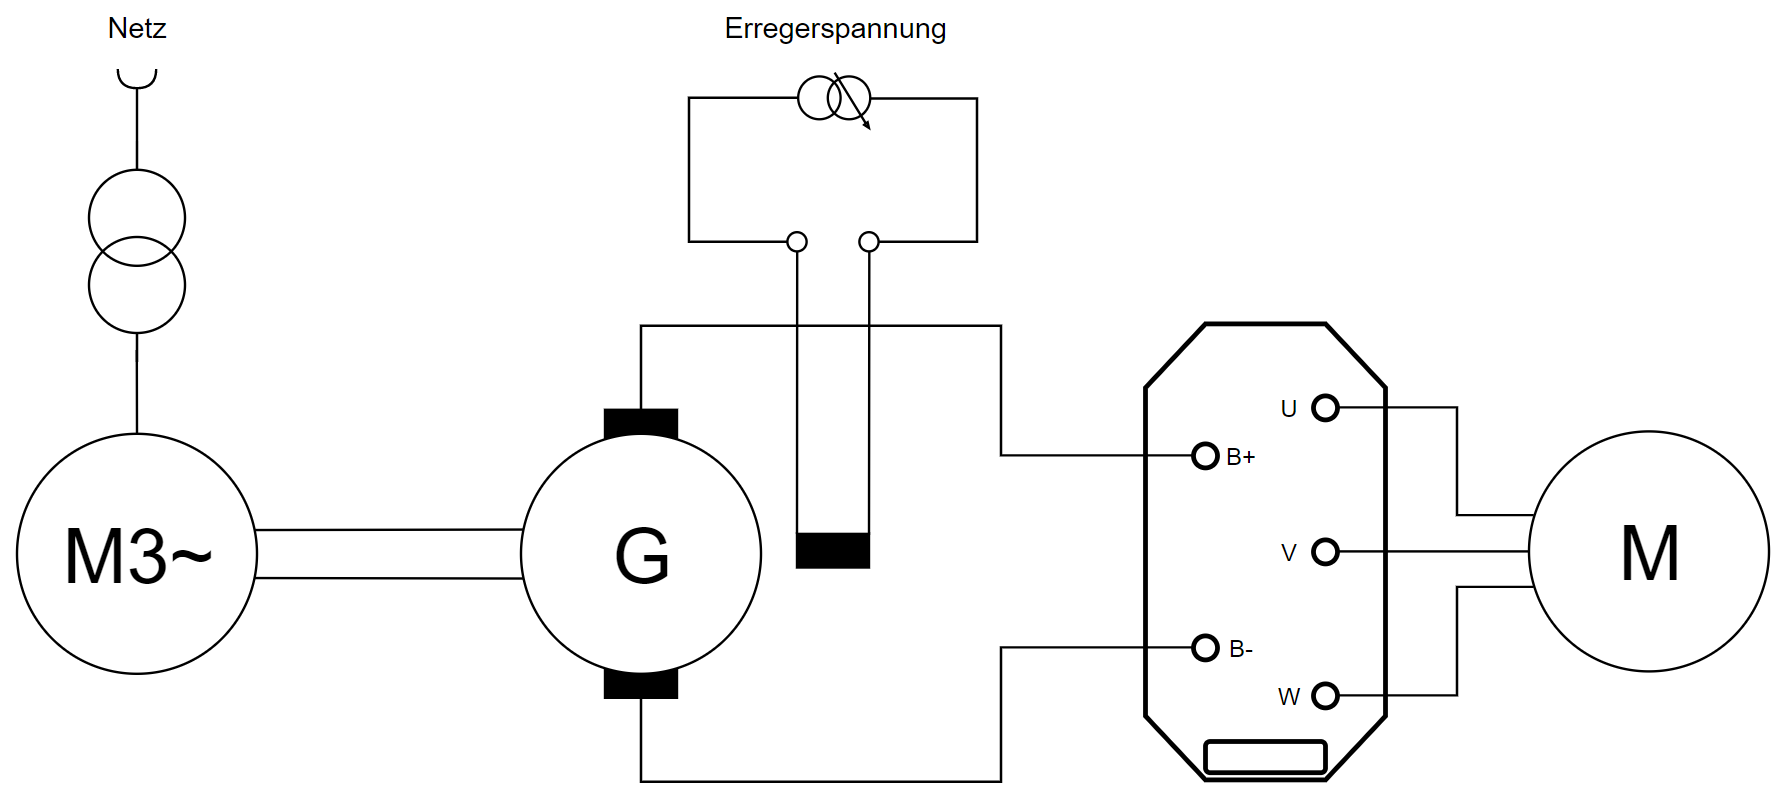
\includegraphics[width=\textwidth]{figures/antrieb/Leonard_Umformer.png}
		\caption{Leonardumformer Versuchsaufbau}
	\end{center}
\end{figure}


\newpage

\subsection{Bleiakku-Versuchsaufbau}

\textbf{Grundidee:}
\\[2mm]
Der Leonard-Veruchsaufbau hat aufgrund der Trägheit der Spannungsquelle nicht funktioniert. Übrig blieb deshalb nur die Realisierung der Spannungsquelle mithilfe eines Ersatz-Akkumulators. Zufälligerweise konnten wir im Projektraum vier Bleiakkumulatoren ausfindig machen, welche wir nun seriell zu einer 48V-Spannungsquelle verschalten wollten. Die Bleiakkus waren zwar teils angeschlagen bzw. sehr tief entladen, mittels eines intelligenten Ladegeräts konnten aber 3 von 4 Akkus wieder erfolgreich aufgeladen werden. Mit einer von Zuhause mitgebrachten Autobatterie und zusätzlichen Starterkabeln konnte letztendlich aber die 48V-Spannungsquelle realisiert werden.
\\[5mm]

\textbf{Fazit:}
\\[2mm]
Der Aufbau mit den Bleiakkumulatoren hat vorübergehend ganz gut funktioniert. Ein Problem stellten vorerst aber die großen Einschaltströme dar, welche bei der Schließung des Stromkreises zu Lichtbögen führten. Um Beschädigungen an den Kondensatoren zu verhindern, konnte dieses Problem jedoch durch Vorladen der Kondensatoren mithilfe eines 48V Netzgerätes behoben werden.
\\[5mm]

\textbf{Erste Inbetriebnahme:}
\\[2mm]
Der Testlauf zur Einstellung der Motorparameter hat mithilfe der Bleiakkumulatoren beim ersten Versuch erfolgreich funktioniert. Der Motor konnte nach weiteren Konfigurationen letztendlich auch eine bestimmte Drehzahl abhängig von einem Spannungssignal anfahren. 


\begin{figure}[H]
	\begin{center}
		%\includegraphics[width=\textwidth]{figures/antrieb/Bleiakku.png}
		\caption{Bleiakku}
	\end{center}
\end{figure}

\newpage

=======
>>>>>>> 909ce2e364172eacda8c0ef77d3e60d4f81ec294
